\lab{Nearest Neighbor Search}{Nearest Neighbor Search}

\objective{The nearest neighbor problem is an optimization problem that arises in applications such as computer vision, pattern recognition, internet marketing, and data compression.
Solving the problem efficiently requires the use of a k-d tree, a variation of the binary search tree.
In this lab we implement a k-d tree, use it to solve the nearest neighbor problem, then apply SciPy's k-d tree object to a handwriting recognition algorithm.}

\section*{The Nearest Neighbor Problem} % =====================================

Suppose you move into a new city with several post offices.
Since your time is valuable, you wish to know which post office is closest to your home.
This is called the nearest neighbor search problem, and it has many applications.

In general, suppose that $X$ is a collection of data, called a \emph{training set}.
Let $y$ be any point (often called the \emph{target} point) in the same space as the data in $X$.
The nearest neighbor search problem determines the point in $X$ that is closest to $y$.
For example, in the post office problem, the set $X$ could be addresses or latitude and longitude data for each post office in the city.
Then $y$ would be the data that represents your new home, and the task is to find the closest post office in $X$ to $y$.

\begin{problem} % Euclidean Distance
Roughly speaking, a function that measures the distance between two points in a set is called a \emph{metric}.\footnote{Metrics and metric spaces are examined in detail in Chapter 5 of Volume I.}
The \emph{Euclidean metric} measures the distance between two points in $\mathbb{R}^n$ with the familiar distance formula:
\[
d(\x,\y) = \sqrt{\displaystyle\sum_{i=1}^n (x_i - y_i)^2} = \| \x - \y \|_2
\]

Write a function that accepts two 1-dimensional NumPy arrays and returns the Euclidean distance between them.
Raise a \li{ValueError} if the arrays don't have the same number of entries.
\\
(Hint: NumPy already has some functions to help do this quickly.)
\end{problem}

Consider again the post office example.
One way to find out which post office is closest is to drive from home to each post office, measure the mileage, and then choose the post office that is the closest.
This is called an \emph{exhaustive search}.
More precisely, measure the distance of $y$ to each point in $X$, and choose the point in $X$ with the smallest distance from $y$.
However, this method is inefficient, and only feasible for relatively small training sets.

\begin{problem} % Exhaustive search method.
Write a function that solves the nearest neighbor search problem by exhaustively checking all of the distances between a given point and each point in a data set.
The function should take in a set of data points (as an $m \times k$ NumPy array, where each row represents one of the $m$ points in the data set) and a single target point (as a 1-dimensional NumPy array with $k$ entries).
Return the point in the training set that is closest to the target point and its distance from the target.

The complexity of this algorithm is $O(mk)$, where $k$ is the number of dimensions and $m$ is the number of data points.
\end{problem}

\section*{K-D Trees} % ========================================================

% \footnote{This lab is a sequel to the Data Structures II lab, and should not be attempted until the reader has successfully implemented a binary search tree in Python.}
A \href{https://en.wikipedia.org/wiki/K-d_tree}{\emph{$k$-d tree}} is a special kind of binary search tree for high dimensional data (i.e., more dimensions than one).
While a binary search tree excludes regions of the number line from a search until the search point is found, a $k$-d tree works on regions of $\mathbb{R}^k$.
In other words, a regular binary search tree partitions $\mathbb{R}$, but a $k$-d tree partitions $\mathbb{R}^{k}$.
So long as the data in the tree meets certain dimensionality requirements, similar efficiency gains may be made.

Recall that to search for a value in a binary search tree, start at the root, and if the value is less than the root, proceed down the left branch of the tree.
If it is larger, proceed down the right branch.
By doing this, a subset of values (and therefore the subtree containing those values) is excluded from the search.
By eliminating this subset from consideration, there are far fewer points to search and the efficiency of the search is greatly increased.
% See Figure \ref{fig:k-binary-search} for an illustration.

Like a binary search tree, a $k$-d tree starts with a root node with a depth, or level, of 0.
At the $i^{th}$ level, the nodes to the left of a parent have a strictly lower value in the $i^{th}$ dimension.
Nodes to the right have a greater or equal value in the $i^{th}$ dimension.
At the next level, do the same for the next dimension.
For example, consider data in $\mathbb{R}^3$.
The root node partitions the data according to the first dimension.
The children of the root partition according to the second dimension, and the grandchildren along the third.
See Figures \ref{fig:kdt-insert} and \ref{fig:k-insert} for examples in $\mathbb{R}^2$ and $\mathbb{R}^3$.

As with any other data structure, the first task is to construct a node class to store data.
A \li{KDTNode} is similar to a \li{BSTNode}, except it has another attribute called \li{axis}.
The \li{axis} attribute indicates the dimension of $\mathbb{R}^k$ to compare points.

\begin{problem} % KDTNode class
Import the \li{BSTNode} class from the previous lab using the following code:
\begin{lstlisting}
import sys
sys.path.insert(1, "../Trees")
from trees import BSTNode
\end{lstlisting}
%\footnote{If the file containing the \li{BSTNode} class is in a different directory than your solutions file for this lab, see \url{https://docs.python.org/2/tutorial/modules.html\#packages} for instructions on packages and imports.}
Write a \li{KDTNode} class that inherits from \li{BSTNode}.
Modify the constructor so that a \li{KDTNode} can only hold a NumPy array (of type \li{np.ndarray}).
If any other data type is given, raise a \li{TypeError}.
Create an \li{axis} attribute (set it to \li{None} or $0$ for now).

\begin{comment} % Magic methods (outdated)
\item Write the \li{__sub__} magic method so that \li{x} - \li{y} returns the Euclidean distance between the data in node \li{x} and the data in node \li{y}.

\item Write the \li{__eq__} magic method so that \li{x == y} is \li{True} if and only if \li{x} and \li{y} have the same data (Hint: \li{np.allclose()})

\item Finally, write the \li{__lt__} and \li{__gt__} magic methods so that the $<$ and $>$ operators compare the $i^{th}$ entry of the data, where $i$ is the \li{axis} attribute of the node on the \emph{right side} of the operator.
For example,

\begin{lstlisting}
>>> x = KDTNode(np.array([1,2]))
>>> y = KDTNode(np.array([3,1]))
>>> y.axis = 0            # Compare the '0th' entry of the data
>>> x < y                # True, since 1 < 3
True
>>> x > y
False

>>> y.axis = 1            # Compare the '1st' entry of the data
>>> x < y                # False, since 2 > 1
False
>>> x > y
True
\end{lstlisting}
\end{comment}
\end{problem}

\begin{figure}[h]
\begin{center}
% Two diagrams as an example of a 2 dimensional KD Tree
% Left diagram
\begin{tikzpicture}[
    level 1/.style={sibling distance=2cm},
    level 2/.style={sibling distance=2cm},
    edge from parent/.style={draw, ->, >=stealth'}]

    % Place the nodes and labels
    \node [draw, circle] (a) {($\underline{\textbf{5}}$,5)}
        child {node[draw, circle] (b) {(3,$\underline{\textbf{2}}$)}
	        child {node[draw = none] (invisble) {} edge from parent[draw=none]}
	        child {node[draw, circle] (c) {($\underline{\textbf{2}}$,6)}}}
        child {node[draw, circle] (d) {(8,$\underline{\textbf{4}}$)}
	        child {node[draw = none] (invisble1) {} edge from parent[draw=none]}
		    child {node[draw, circle] (e) {($\underline{\textbf{7}}$,7)}}};

    % Guiding remarks
    \node [draw=none, black!20!blue, node distance=1.5cm] (1) [above right of=a] {check dimension 1};
    \draw[black!20!blue, ->, >=stealth', shorten >= .1cm] (1)--(a);
    \node [draw=none, black!20!blue, node distance=1.5cm] (2) [above right of=d] {check dimension 2};
    \draw[black!20!blue, ->, >=stealth', shorten >= .1cm] (2)--(d);
\end{tikzpicture}
\qquad
% Right diagram
\begin{tikzpicture}[
	level 1/.style={sibling distance=3.5cm},
	level 2/.style={sibling distance=2cm},
	edge from parent/.style={draw, ->, >=stealth'}]

	% Place the nodes and labels
	\node [draw, circle] (a) {($\underline{\textbf{5}}$,5)}
		child {node[draw, circle] (b) {(3,$\underline{\textbf{2}}$)}
			child {node[draw = none] (invisble) {} edge from parent[draw=none]}
			child {node[draw, circle] (d) {($\underline{\textbf{2}}$,6)}}}
		child {node[draw, circle] (c) {(8,$\underline{\textbf{4}}$)}
			child {node[draw, circle] (e) {($\underline{\textbf{9}}$,2)}}
			child {node[draw, circle] (f) {($\underline{\textbf{7}}$,7)}}};

	% Guiding remarks
	\node [draw=none, black!20!blue, node distance=1.5cm] (1) [above left of=e] {insert};
	\draw[black!20!blue, ->, >=stealth', shorten >= .1cm] (1)--(e);
\end{tikzpicture}
\end{center}
\caption{These trees illustrate an insertion of (9, 2) into a $k$-d tree in $\mathbb{R}^2$ loaded with the points (5, 5), (8, 4), (3, 2), (7, 7), and (2, 6), in that order. To insert the point (9, 2), find the node that will be the new node's parent. Start at the root. Since the $x$-coordinate of (9, 2) is greater than the $x$-coordinate of (5, 5), move into the right subtree of the root node, thus excluding all points ($x$, $y$) with $x < 5$. Next, compare (9, 2) to the root's right child, (8, 4). Since the $y$-coordinate of (9, 2) is less than the $y$-coordinate of (8, 4), move to the left of (8,4), thus excluding all points ($x$, $y$) with $y > 4$. Since (8,4) does not have a left child, insert (9, 2) as the left child of (8,4).}
\label{fig:kdt-insert}
\end{figure}

\begin{figure}[H]
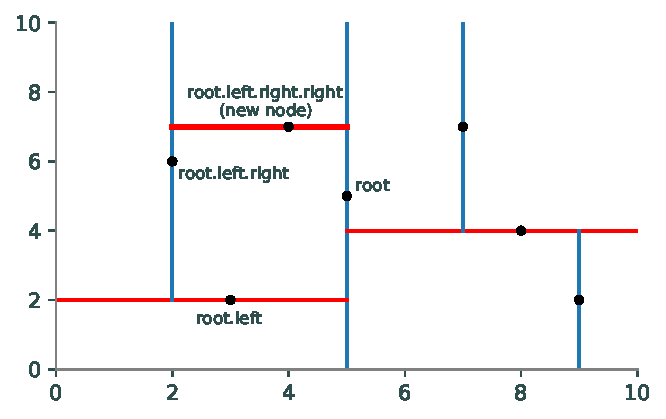
\includegraphics[width=.9\textwidth]{figures/kdpic5.pdf}
\caption{This figure is another illustration of the $k$-d tree from Figure \ref{fig:kdt-insert} with the point (9,2) already inserted. To insert the point (4, 7), start at the root. Since the $x$-coordinate of (4, 7) is less than the $x$-coordinate of (5, 5), move into the region to the left of the middle blue line, to the root's left child, (3, 2). The $y$-coordinate of (4, 7) is greater than the $y$-coordinate of (3, 2), so move above the red line on the left, to the right child (2, 6). Now return to comparing the $x$-coordinates, and since $4 > 2$ and (2, 6) has no right child, install (4, 7) as the right child of (2, 6).}
\label{fig:k-insert}
\end{figure}

% old picture with old caption
\begin{comment}
\begin{figure}[H]
\includegraphics[width=.7\textwidth]{figures/kdpic2.png}
\caption{To insert the point (4, 7) into the $k$-d tree of Figure \ref{fig:k-binary-search}, find the node that will be the new node's parent. Start at the root, (5, 5). Since the $x$-coordinate of (4, 7) is less than the $x$-coordinate of (5, 5), move into the region to the left of the middle blue line, to the root's left child, (3, 2). The $y$-coordinate of (4, 7) is greater than the $y$-coordinate of (3, 2), so move above the red line on the left, to the right child (2, 6). Now return to comparing the $x$-coordinates, and since $4 > 2$ and (2, 6) has no right child, install (4, 7) as the right child of (2, 6).}
\label{fig:k-insert}
\end{figure}
\end{comment}

\begin{comment} % KDT Node class
\begin{lstlisting}
# import the BSTNode class from the previous lab.

class KDTNode(BSTNode):
    """Node class for K-D Trees. Inherits from BSTNode.
    Attributes:
        left (KDTNode): a reference to this node's left child.
        right (KDTNode): a reference to this node's right child.
        parent (KDTNode): a reference to this node's parent node.
        data (ndarray): a coordinate in k-dimensional space.
        axis (int): the dimension to make comparisons on.
    """
    def __init__(self, data):
        """Construct a K-D Tree node containing 'data'. The left, right,
        and prev attributes are set in the constructor of BSTNode.
        """
        BSTNode.__init__(self, data)
        self.axis  = 0
\end{lstlisting}
\end{comment}

% Now we construct the $k$-d tree class.
% For an optimal $k$-d tree, the data needs to be inserted in a very particular order.
% However, inserting at random still usually produces a good tree.
% Here we simply insert the data in the order that it is given.
% TODO: put this elsewhere (in the problem statement?).

The major difference between a $k$-d tree and a binary search tree is how the data is compared at each depth level.
Though the nearest neighbor problem does not need to use a \li{find()} method, the $k$-d tree version of \li{find()} is provided as an instructive example.

In the \li{find()} method, every comparison in the recursive \li{_step()} function compares the data of \li{target} and \li{current} based on the \li{axis} attribute of \li{current}.
This way, if each existing node in the tree has the correct \li{axis}, the correct comparisons are made when descending through the tree.

\begin{figure}[H]
\begin{center}
%Example of a 3 dimensional KD Tree
\begin{tikzpicture}[
	level 1/.style={sibling distance=7cm},
	level 2/.style={sibling distance=4cm},
	level 3/.style={sibling distance=3cm},
	level 4/.style={sibling distance=3cm},
	edge from parent/.style={draw, ->, >=stealth'}]

	%Place the nodes and labels
	\node [draw, circle] (a) {($\underline{\textbf{3}}$,1,4)}
		child {node[draw, circle] (b) {(2,$\underline{\textbf{3}}$,7)}
			child {node[draw, circle] (c) {(2,1,$\underline{\textbf{3}}$)}}
			child {node[draw, circle] (d) {(2,4,$\underline{\textbf{5}}$)}
				child {node[draw, circle] (e) {($\underline{\textbf{1}}$,4,4)}}
				child {node[draw, circle] (f) {($\underline{\textbf{0}}$,5,7)}}}}
		child {node[draw, circle] (g) {(4,$\underline{\textbf{3}}$,4)}
			child {node[draw, circle] (h) {(6,1,$\underline{\textbf{4}}$)}
				child {node[draw = none] (invisble) {} edge from parent[draw=none]}
				child {node[draw, circle] (i) {($\underline{\textbf{5}}$,2,5)}
					child {node[draw, circle] (j) {(4,$\underline{\textbf{0}}$,6)}}
					child {node[draw, circle] (k) {(7,$\underline{\textbf{1}}$,6)}}}}
			child {node[draw = none] (invisble1) {} edge from parent[draw=none]}};

	%Guiding remarks
	\node [draw=none, black!20!blue, node distance=1.5cm] (1) [above right of=a] {check dimension 1};
	\draw[black!20!blue, ->, >=stealth', shorten >= .1cm] (1)--(a);
	\node [draw=none, black!20!blue, node distance=1.5cm] (2) [above of=g] {check dimension 2};
	\draw[black!20!blue, ->, >=stealth', shorten >= .1cm] (2)--(g);
	\node [draw=none, black!20!blue, node distance=1.5cm] (3) [above left of=h] {check dimension 3};
	\draw[black!20!blue, ->, >=stealth', shorten >= .1cm] (3)--(h);
	\node [draw=none, black!20!blue, node distance=1.5cm] (4) [above right of=i] {back to dimension 1};
	\draw[black!20!blue, ->, >=stealth', shorten >= .1cm] (4)--(i);
	\node [draw=none, black!20!blue, node distance=1.5cm] (5) [above right of=k] {check dimension 2};
	\draw[black!20!blue, ->, >=stealth', shorten >= .1cm] (5)--(k);
\end{tikzpicture}
\end{center}
\caption{To find the point (7, 1, 6), start at the root. Since the $x$-coordinate of (7, 1, 6) is greater than the $x$-coordinate of (3, 1, 4), move to the right subtree of the root node, thus excluding all points ($x$, $y$, $z$) with $x < 7$. Next, compare (7, 1, 6) to the root's right child, (4, 3, 4). Since the $y$-coordinate of (7, 1, 6) is less than the $y$-coordinate of (4, 3, 4), move to the left subtree of (4, 3, 4), thus excluding all points ($x$, $y$, $z$) with $y > 1$. Continue in this manner until (7, 1, 6) is found.} % Next, compare (7, 1, 6) to (6, 1, 4), the left child of (4, 3, 4). Since the $z$-coordinate of (7, 1, 6) is greater than the $z$-coordinate of (6, 1, 4), move to the right subtree of (6, 1, 4). Now, when comparing (5, 2, 5) with (7, 1, 6), start back at the first dimension. Since the $x$-coordinate of (7, 1, 6) is greater than the $x$-coordinate of (5, 2, 5), move to the right child of (5, 2, 5). The point (7, 1, 6) is found, since it is the right child of (5, 2, 5).}
\label{fig:kdt-find}
\end{figure}

\begin{lstlisting}
import numpy as np
# Import the BST class from the previous lab.
import sys
sys.path.insert(1, "../Trees")
from trees import BST

class KDT(BST):
    """A k-dimensional binary search tree object.
    Used to solve the nearest neighbor problem efficiently.

    Attributes:
        root (KDTNode): The root node of the tree. Like all nodes in the tree,
            the root houses data as a NumPy array.
        k (int): The dimension of the tree (the 'k' of the k-d tree).
    """

    def find(self, data):
        """Return the node containing 'data'. If there is no such node in the
            tree, or if the tree is empty, raise a ValueError.
        """

        # Define a recursive function to traverse the tree.
        def _step(current):
            """Recursively step through the tree until the node containing
            'data' is found. If there is no such node, raise a Value Error.
            """
            if current is None:                     # Base case 1: dead end.
                raise ValueError(str(data) + " is not in the tree")
            elif np.allclose(data, current.value):
                return current                      # Base case 2: data found!
            elif data[current.axis] < current.value[current.axis]:
                return _step(current.left)          # Recursively search left.
            else:
                return _step(current.right)         # Recursively search right.

        # Start the recursion on the root of the tree.
        return _step(self.root)
\end{lstlisting}

% \begin{comment}
\begin{figure}[H]
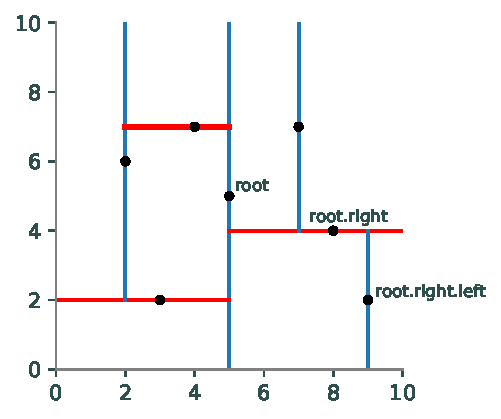
\includegraphics[width=.7\textwidth]{figures/kdpic4_equal.pdf}
\caption{The above graph is another illustration of the $k$-d tree from Figure \ref{fig:kdt-insert}. To find the point (9, 2), start at the root. Since the $x$-coordinate of (9, 2) is greater than the $x$-coordinate of (5, 5), move into the region to the right of the middle blue line, thus excluding all points ($x$, $y$) with $x < 5$. Next, compare (9, 2) to the root's right child, (8, 4). Since the $y$-coordinate of (9, 2) is less than the $y$-coordinate of (8, 4), move below the red line on the right, thus excluding all points ($x$, $y$) with $y > 4$. The point (9, 2) is now found, since it is the left child of (8, 4).}
\label{fig:k-binary-search}
\end{figure}
% \end{comment}

\begin{problem} % Implement the K-D Tree!
Finish implementing the \li{KDT} class.
\begin{enumerate}
\item Override the \li{insert()} method.
To insert a new node, find the node that should be the parent of the new node by recursively descending through the tree as in the \li{find()} method (see Figure \ref{fig:k-insert} for a geometric example).
Do not allow duplicate nodes in the tree.
Note that the \li{k} attribute will be initialized when a $k$-d tree object is instantiated.

The \li{axis} attribute of the new node will be one more than that axis of the parent node.
If the last dimension of the data has been reached, start \li{axis} over at 0.

\item % To solve the nearest neighbor search problem, create the $k$-d tree only once.
% Then use it multiple times with different target points.
To prevent a user from altering the tree, disable the \li{remove()} method.
Raise a \\ \li{NotImplementedError} if the method is called, and allow it to receive any number of arguments.
(Disabling the \li{remove()} method ensures that the $k$-d tree remains the same after it is created.
The same $k$-d tree is used multiple times with different target points to solve the nearest neighbor search problem.)
\end{enumerate}
\end{problem}

Using a $k$-d tree to solve the nearest neighbor search problem requires some care.
At first glance, it appears that a procedure similar to \li{find()} or \li{insert()} will immediately yield the result.
However, this is not always the case (see Figure \ref{fig:bad-search}).

To correctly find the nearest neighbor, keep track of the target point, the current search node, current best point, and current minimum distance.
Start at the root node.
Then the current search node and current best point will be root, and the current minimum distance will be the Euclidean distance from \li{root} to \li{target}.
Then proceed recursively as in the \li{find()} method.
As closer points (nearer neighbors) are found, update the appropriate variables accordingly.

Once the bottom of the tree is reached, a "close" neighbor has been found.
However, this is not guaranteed to be the closest point.
One way to ensure that this is the closest point is to draw a hypersphere with a radius of the current minimum distance around the candidate nearest neighbor.
If this hypersphere does not intersect any of the hyperplanes that split the $k$-d tree, then this is indeed the closest point.

\begin{figure}[H]
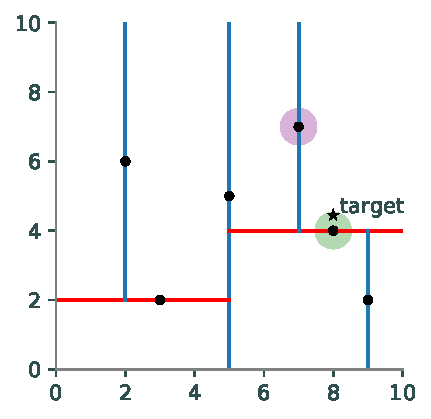
\includegraphics[width=.7\textwidth]{figures/kdpic6.pdf}
\caption{To find the point in the $k$-d tree of Figure \ref{fig:k-insert} that is closest to (8, 4.5), first record the distance from the root to the target as the current minimum distance (about 3.04). Then travel down the tree to the right. The right child, (8, 4), is only 0.5 units away from the target (the green circle), so update the minimum distance. Since (8, 4) is not a leaf in the tree, the algorithm could continue down to the left child, (7, 7). However, this leaf node is much further from the target (the purple circle). To ensure that algorithm terminates correctly, check to see if the hypersphere of radius 0.5 around the current node (the green circle) intersects with any other hyperplanes. Since it does not, stop descending down the tree and conclude (correctly) that (8, 4) is the nearest neighbor.}
\label{fig:bad-search}
\end{figure}

While the correct hypersphere cannot be easily drawn, there is an equivalent procedure that has a straightforward implementation in Python.
Before deciding to descend in one direction, add the minimum distance to the $i^{th}$ entry of the target point's data, where $i$ is the \li{axis} of the candidate nearest neighbor.
If this sum is greater that the $i^{th}$ entry of the current search node, then the hypersphere would necessarily intersect one of the hyperplanes drawn by the tree (why?).

The algorithm is summarized below.

\begin{algorithm}[h] % K-d search algorithm.
\begin{algorithmic}[1]
\State Given a set of data and a \texttt{target}, build a $k$-d tree out of the data set.
\Procedure{Search}{\texttt{current, neighbor, dist}}
\If {\texttt{current} is \texttt{None}}
    \Comment{Base case.}
    \State \pseudoli{return} \texttt{neighbor, dist}
\EndIf
\State \texttt{index} $\gets$ \texttt{current.axis}
\If {metric(\texttt{current, target}) $<$ \texttt{dist}}
    \State \texttt{neighbor} $\gets$ \texttt{current}
        \Comment{Update the best estimate.}
    \State \texttt{dist} $\gets$ metric(\texttt{current, target})
\EndIf
\If {\texttt{target[index]} $<$ \texttt{current.value[index]}}
    \Comment{Recurse left.}
    \State \texttt{neighbor, dist} $\gets$ Search(\texttt{current.left, neighbor, dist})
    \If {\texttt{target[index]} + \texttt{dist} $\geq$ \texttt{current.value[index]}}
        \State \texttt{neighbor, dist} $\gets$ Search(\texttt{current.right, neighbor, dist})
    \EndIf
\Else
    \Comment{Recurse right.}
    \State \texttt{neighbor, dist} $\gets$ Search(\texttt{current.right, neighbor, dist})
    \If{\texttt{target[index]} - \texttt{dist} $\leq$ \texttt{current.value[index]}}
        \State \texttt{neighbor, dist} $\gets$ Search(\texttt{current.left, neighbor, dist})
    \EndIf
\EndIf
\State \pseudoli{return} \texttt{neighbor, dist}
\EndProcedure
\State Start \textsc{Search()} at the root of the tree.
\end{algorithmic}
\caption{$k$-d tree nearest neighbor search}
\label{alg:kdneighborz}
\end{algorithm}

\begin{problem} % K-d nearest neighbor search algorithm.
Use Algorithm \ref{alg:kdneighborz} to write a function that solves the nearest neighbor search problem by searching through your \li{KDT} object.
The function should take in a NumPy array of data and a NumPy array representing the target point.
Return the nearest neighbor in the data set and the distance from the nearest neighbor to the target point, as in Problem 2 (be sure to return a NumPy array for the neighbor).

To test your function, use SciPy's built-in \li{KDTree} object.
This structure behaves like the \li{KDT} class, but its operations are heavily optimized.
To solve the nearest neighbor problem, initialize the tree with data, then ``query'' the tree with the target point.
The \li{query()} method returns a tuple of the minimum distance and the index of the nearest neighbor in the data.

\begin{lstlisting}
>>> from scipy.spatial import KDTree

# Initialize the tree with data (in this example, use random data).
>>> data = np.random.random((100,5))
>>> target = np.random.random(5)
>>> tree = KDTree(data)

# Query the tree and print the minimum distance.
>>> min_distance, index = tree.query(target)
>>> print(min_distance)
0.309671532426

# Print the nearest neighbor by indexing into the tree's data.
>>> print(tree.data[index])
[ 0.68001084  0.02021068  0.70421171  0.57488834  0.50492779]
\end{lstlisting}
\end{problem}

\section*{$k$-Nearest Neighbors}
Previously in the lab, a $k$-d tree was used to find the nearest neighbor of a target point.
A more general problem is to find the \emph{k} nearest neighbors to a point for some $k$ (using some metric to measure ``distance'' between data points).
The $k$-nearest neighbors algorithm is a machine learning model. % that tries to correctly classify unknown data points based on the classifications of known data points.
In machine learning, a set of data points has a corresponding set of \emph{labels}, or classifications, that specifies the category of a specific data point in the training set.
A machine learning algorithm takes unlabelled data and learns how to classify it.
For example, suppose a data set contains the incomes and debt levels of $n$ individuals.
Along with this data, there is a set of $n$ data points that state whether an individual has filed for bankruptcy; these points are the labels.
The goal of a machine learning model would be to correctly predict whether a new individual would go bankrupt.
% These assignments are made based on a set of data points with corresponding \emph{labels}. The labels are the classifications of those data points.
% Relationships between a new data point and the set of labeled data points determine the classification of the new data point.

\subsection*{Classification}
In classification, the $k$ nearest neighbors of a new point are found, and each neighbor ``votes'' to decide what label to give the new point.
The ``vote'' of each neighbor is its label, or output class.
The output class with the highest number of votes determines the label of the new point.
See Figure \ref{fig:knn} for an illustration of the algorithm.

Consider the bankruptcy example.
If the 10 nearest neighbors to a new individual are found and 8 of them went bankrupt, then the algorithm would predict that the individual would also go bankrupt.
On the other hand, if 7 of the nearest neighbors had not filed for bankruptcy, the algorithm would predict that the individual was at low risk for bankruptcy.

\begin{figure}[h]
\begin{center}
\begin{tikzpicture}[circ/.style={circle,thick,align=center,minimum size=1.5cm,text=black,font=\Huge}]
% Red node
\node[circ,red,fill=red] (R) {};
% Blue nodes
\node[cyan!70,fill=cyan!70,circ,above left=.5cm and .5cm of R] (B1) {$\textbf{A}$};
\node[cyan!70,fill=cyan!70,circ,below left=.25cm and 3cm of R] (B2) {$\textbf{A}$};
\node[cyan!70,fill=cyan!70,circ,below left=-.5cm and .9cm of R] (B3) {$\textbf{A}$};
\node[cyan!70,fill=cyan!70,circ,below left=1.4cm and .6cm of R] (B4) {$\textbf{A}$};
%Yellow nodes
\node[yellow!60,fill=yellow!60,circ,above right=1.7cm and 2cm of R] (Y1) {$\textbf{B}$};
\node[yellow!60,fill=yellow!60,circ,above right=.5cm and .5cm of R] (Y2) {$\textbf{B}$};
\node[yellow!60,fill=yellow!60,circ,below right=0cm and 1.5cm of R] (Y3) {$\textbf{B}$};
% Green nodes
\node[green!30,fill=green!95!black,circ,above right=-.5cm and 2.5cm of R] (G1) {$\textbf{C}$};
\node[green!30,fill=green!95!black,circ,below right=4cm and 0cm of R] (G2) {$\textbf{C}$};
\node[green!30,fill=green!95!black,circ,below right=2cm and .4cm of R] (G3) {$\textbf{C}$};
\node[green!30,fill=green!95!black,circ,below right=3cm and 1.75cm of R] (G4) {$\textbf{C}$};
\node[green!30,fill=green!95!black,circ,below right=1.75cm and 3cm of R] (G5) {$\textbf{C}$};
% Lines
\foreach \a/\b in {R/B1,R/B3,R/Y2} \draw[line width=.1cm] (\a) -- (\b);
\end{tikzpicture}
\caption{In this example, the red node is the new point that needs to be classified. Its three nearest neighbors are two type A nodes and one type B node. The red node is classified as type A since that is the most common label of its three nearest neighbors.}
\label{fig:knn}
\end{center}
\end{figure}

\begin{comment}
To determine the accuracy of a machine learning model, first divide the set of labeled data into a \emph{training set} and a \emph{test set}.
The training set is used to find potentially predictive relationships between the \emph{features}, or individual properties, of a data point.
In the bankruptcy example above, the incomes and debt levels were features of the data.
Relationships between features are discovered in the \emph{training phase} of machine learning.
In the nearest neighbor algorithm, the training phase consists of simply storing the training set.
The test set is a small subset (usually around 20\%) of the original data set.
During the \emph{test phase}, the accuracy of the model is calculated using the test set.
The test set is treated as a set of novel data, and is run through the model.
The model's classifications of the test data are compared to the actual labels of the test data.
The ratio of correct classifications to total number of instances in the test set is the accuracy of the model.
\end{comment}

\begin{comment}
\subsection*{Breaking Ties}
Consider the illustration in Figure \ref{fig:knn}.
Suppose that the three neighbors of a new data point were found, but all of these neighbors had different classifications: one neighbor was of class A, one was B, and one was C.
How would the new instance be classified?
A common approach to dealing with ties is to remove the farthest neighbor's vote until a majority vote is found.
In some cases, this results in only the closest neighbor determining the output of a new instance.
\end{comment}

\subsection*{Handwriting Recognition} % ---------------------------

The problem of recognizing handwritten letters and numbers with a computer has many applications.
A computer image may be thought of as a vector in $\mathbb{R}^n$, where $n$ is the number of pixels in the image and the entries represent how bright each pixel is.
If two people write the same number, the vectors representing a scanned image of those numbers are expected to be close in the Euclidean metric.
This insight means that given a training set of scanned images along with correct labels, the label of a new scanned image can be confidently inferred.

\begin{problem} % Postal data problem.
Write a class that performs the $k$-nearest neighbors algorithm.
The constructor should accept a NumPy array of data (the training set) and a NumPy array of corresponding labels for that data.
Use SciPy's \li{KDTree} class to build a $k$-d tree from the training set in the constructor.

Write a method for this class that accepts a NumPy array of new data points and an integer \li{k}.
Use the $k$-nearest neighbors algorithm to predict the label of the new data points.
Return a NumPy array of the predicted labels.
In the case of ties between labels, choose the label with the smaller identifier (hint: try \li{scipy.stats.mode()}).

To test your classifier, use the data file \texttt{PostalData.npz}.
This is a collection of labeled handwritten digits that the United States Postal Service has made available to the public.
This data set may be loaded by using the following command:
\begin{lstlisting}
points, testpoints, labels, testlabels = np.load('PostalData.npz').items()
\end{lstlisting}

The first entry of each array is a name, so \li{points[1]} and \li{labels[1]} are the actual points and labels to use.
Each point is an image that is represented by a flattened $28 \times 28$ matrix of pixels (so each image is a NumPy array of length 784).
The corresponding label indicates the number written and is represented by an integer.

Use \li{labels[1]} and \li{points[1]} to initialize the classifier. Use \li{testpoints[1]} for predicting output classes. Choose a random data point from \li{testpoints[1]}. Plot this point with the following code:
\begin{lstlisting}
import matplotlib.pyplot as plt
plt.imshow(img.reshape((28,28)), cmap="gray")
plt.show()
\end{lstlisting}
where \li{img} is the random data point (a NumPy array of length 784). Your plot should look similar to Figure \ref{fig:digit}.

Use your classifier to predict the label of this data point.
Does the output match the number you plotted?
Compare the output of your classifier to the corresponding label in \li{testlabels[1]}.
They should be the same.

\begin{comment}
The United States Postal Service has made a collection of labeled handwritten digits available to the public, provided in \texttt{PostalData.npz}.
Write a function that uses this data for $k$-nearest neighbor classification.
This data set may be loaded by using the following command:

\begin{lstlisting}
labels, points, testlabels, testpoints = np.load('PostalData.npz').items()
\end{lstlisting}

This contains a training set and a test set.
The first entry of each array is a name, so \li{labels[1]} and \li{points[1]} are the actual points and labels to use.
Each point is an image that is represented by a flattened $28 \times 28$ matrix of pixels (so each image is represented by a NumPy array of length 784).
The corresponding label indicates the number written, and is represented by an integer.

Use SciPy's \li{KDTree} class to build a $k$-d tree from the training set of digits. Perform the $k$-nearest neighbor algorithm on the first 50 nodes in \li{testpoints} using 1, 4, and 10 neighbors, with tie breaking implemented as described above (hint: try using \li{np.bincount()}). Calculate the accuracy of your model by comparing your output to the corresponding labels in \li{testlabels}. Return the accuracies of your model.
\end{comment}

A similar classification process is used by the United States Postal Service to automatically determine the zip code written or printed on a letter.

\begin{figure}[H]
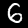
\includegraphics[width=.25\textwidth]{figures/Example.png}
\caption{The number 6 taken from the data set.}
\label{fig:digit}
\end{figure}
\end{problem}

\newpage

\section*{Additional Material}

\subsection*{sklearn}
The \li{sklearn} package contains powerful tools for solving the nearest neighbor problem.
To start nearest neighbors classification, import the \li{neighbors} module from \li{sklearn}.
This module has a class for setting up a $k$-nearest neighbors classifier.

\begin{lstlisting}
# Import the neighbors module
>>> from sklearn import neighbors

# Create an instance of a k-nearest neighbors classifier.
# 'n_neighbors' determines how many neighbors to find.
# 'weights' may be 'uniform' or 'distance.'  The 'distance' option
#     gives nearer neighbors a more weighted vote.
# 'p=2' instructs the class to use the Euclidean metric.
>>> nbrs = neighbors.KNeighborsClassifier(n_neighbors=8, weights='distance', p=2)
\end{lstlisting}

The \li{nbrs} object has two useful methods for classification.
The first, \li{fit}, takes arrays of data (the training set) and labels and puts them into a $k$-d tree.
This is used to find the $k$-nearest neighbors, much like the \li{KDT} class implemented previously in the lab.

\begin{lstlisting}
# 'points' is some NumPy array of data
# 'labels' is a NumPy array of labels describing the data in points.
>>> nbrs.fit(points, labels)
\end{lstlisting}

The second method, \li{predict}, does a k-nearest neighbor search on the $k$-d tree and uses the result to attach a label to unlabeled points.

\begin{lstlisting}
# 'testpoints' is an array of unlabeled points.
# Perform the search and calculate the accuracy of the classification.
>>> prediction = nbrs.predict(testpoints)
>>> nbrs.score(testpoints, testlabels)
\end{lstlisting}

More information about this module can be found at \url{http://scikit-learn.org/stable/modules/neighbors.html}.

\begin{comment}
\newpage

\section*{Additional Material} % ==============================================

% TODO (there's already some material on this in the oldLab/ folder)
\subsection*{The Curse of Dimensionality} % -----------------------------------

\end{comment}
